\section{Công nghệ Backend}
Hệ thống Backend được xây dựng dựa trên nền tảng Node.js, sử dụng ngôn ngữ TypeScript để
đảm bảo tính chặt chẽ của mã nguồn cùng với framework Express.js để xử lý các yêu cầu HTTP
\subsection{Môi trường thực thi: Node.js}
Node.js là một môi trường runtime mã nguồn mở, đa nền tảng, cho phép thực thi JavaScript
bên ngoài trình duyệt web, dựa trên \textbf{V8 JavaScript engine} của Chrome. Điểm khác biệt
cốt lõi của Node.js so với các nền tảng máy chủ truyền thống nằm ở kiến trúc hướng sự kiện
(Event-driven):
\begin{itemize}
    \item \textbf{Single-threaded:} Node.js sử dụng một luồng chính duy nhất để xử lý các kết nối, giúp tiết kiệm tài nguyên hệ thống (RAM, CPU) so với mô hình đa luồng truyền thống.
    \item \textbf{Non-blocking I/O:} Khi gặp các tác vụ nặng về I/O (như đọc file, truy vấn Database), Node.js sẽ không dừng lại chờ đợi (block) mà đẩy tác vụ đó xuống hệ thống xử lý nền, sau đó tiếp tục xử lý các yêu cầu khác.
\end{itemize}

\begin{figure}[H]
    \centering
    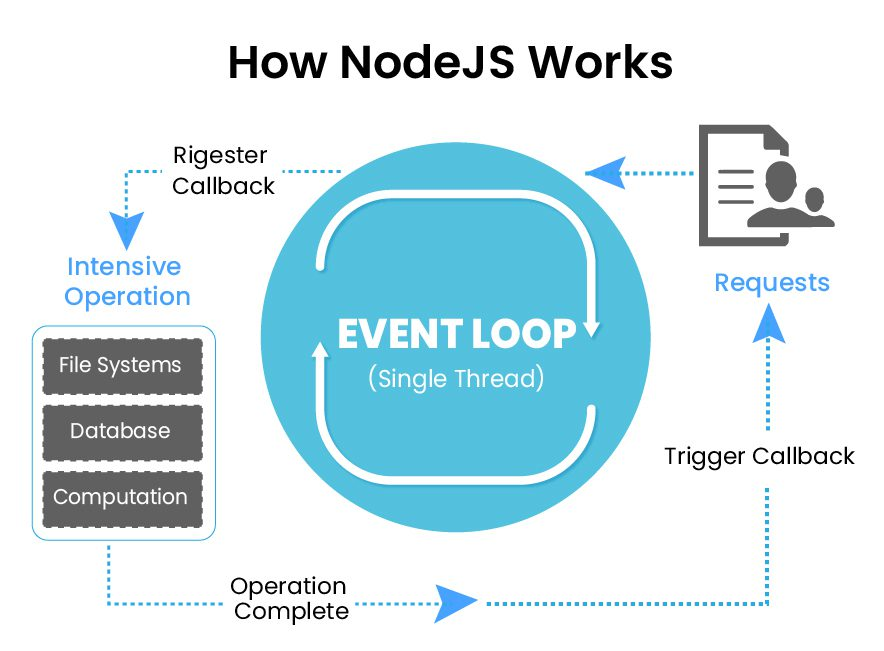
\includegraphics[width=0.7\textwidth]{img/nodejs-architecture.jpg}
    \caption{\textit{Mô hình hoạt động Event Loop của Node.js}}
    \label{fig:nodejs_arch}
\end{figure}

Đối với đề tài này, \textbf{Node.js} là một lựa chọn hiệu quả. Tuy nhiên đối với các
hệ thống khác với những tác vụ tính toán nặng (AI, xử lý ảnh, data mining)
sẽ khiến Event Loop bị nghẽn, làm chậm toàn bộ hệ thống.

\subsection{Ngôn ngữ lập trình: TypeScript}
TypeScript là một ngôn ngữ lập trình mã nguồn mở được phát triển bởi Microsoft, đóng vai trò
là một siêu tập (Superset) của JavaScript.
\begin{itemize}
    \item \textbf{Static Typing:} TypeScript bổ sung hệ thống kiểu dữ liệu tĩnh (Static Types) vào Java\-Script. Các kiểu dữ liệu được kiểm tra ngay tại thời điểm biên dịch (Compile\-time), giúp phát hiện sớm các lỗi sai lệch kiểu dữ liệu trước khi ứng dụng được chạy.
    \item \textbf{Non-blocking I/O:} Cung cấp các cấu trúc lập trình hướng đối tượng nâng cao như
          Interface, Class và Generics, giúp định nghĩa rõ ràng các DTO (Data Transfer Object) và
          cấu trúc dữ liệu trả về từ API.
\end{itemize}

\subsection{ExpressJS Framework}
ExpressJS là một Framework ứng dụng web (Web Application Framework) tối giản và linh hoạt được xây dựng trên nền tảng Node.js. Nó cung cấp một bộ các tính năng mạnh mẽ để phát triển ứng dụng web và API. Express.js đã trở thành framework backend phổ biến
nhất trong hệ sinh thái Node.js nhờ kiến trúc đơn giản, hiệu suất cao và khả
năng mở rộng dễ dàng.

\begin{figure}[H]
    \centering
    
\includegraphics[width=0.7\linewidth]{img/expressjs.jpg}
    \caption{\textit{ExpressJS Framework}}
    \label{fig:express}
\end{figure}

\subsubsection{Các thành phần cốt lõi}
\begin{itemize}
    \item \textbf{Middleware:} Là các hàm có quyền truy cập vào đối tượng yêu cầu (req), đối tượng phản hồi (res) và hàm middleware tiếp theo trong chu trình xử lý (next). Middleware dùng để xử lý logic, xác thực người dùng, log dữ liệu, v.v.
    \item \textbf{Routing:} Cơ chế xác định cách ứng dụng phản hồi các yêu cầu từ client đến một endpoint cụ thể (URI) bằng các phương thức HTTP (GET, POST, PUT, DELETE).
    \item \textbf{Template Engine:} Hỗ trợ tích hợp các template engine như EJS, Pug để render giao diện phía server (nếu cần).
\end{itemize}

\subsubsection{Vai trò trong hệ thống}
Express.js đóng vai trò điều phối luồng dữ liệu, xử lý logic nghiệp vụ API (RESTful API) trước khi tương tác với cơ sở dữ liệu.